\begin{frame}{Bestes Modell und Uebergabe}
\begin{columns}[T,onlytextwidth]
\begin{column}{0.48\textwidth}
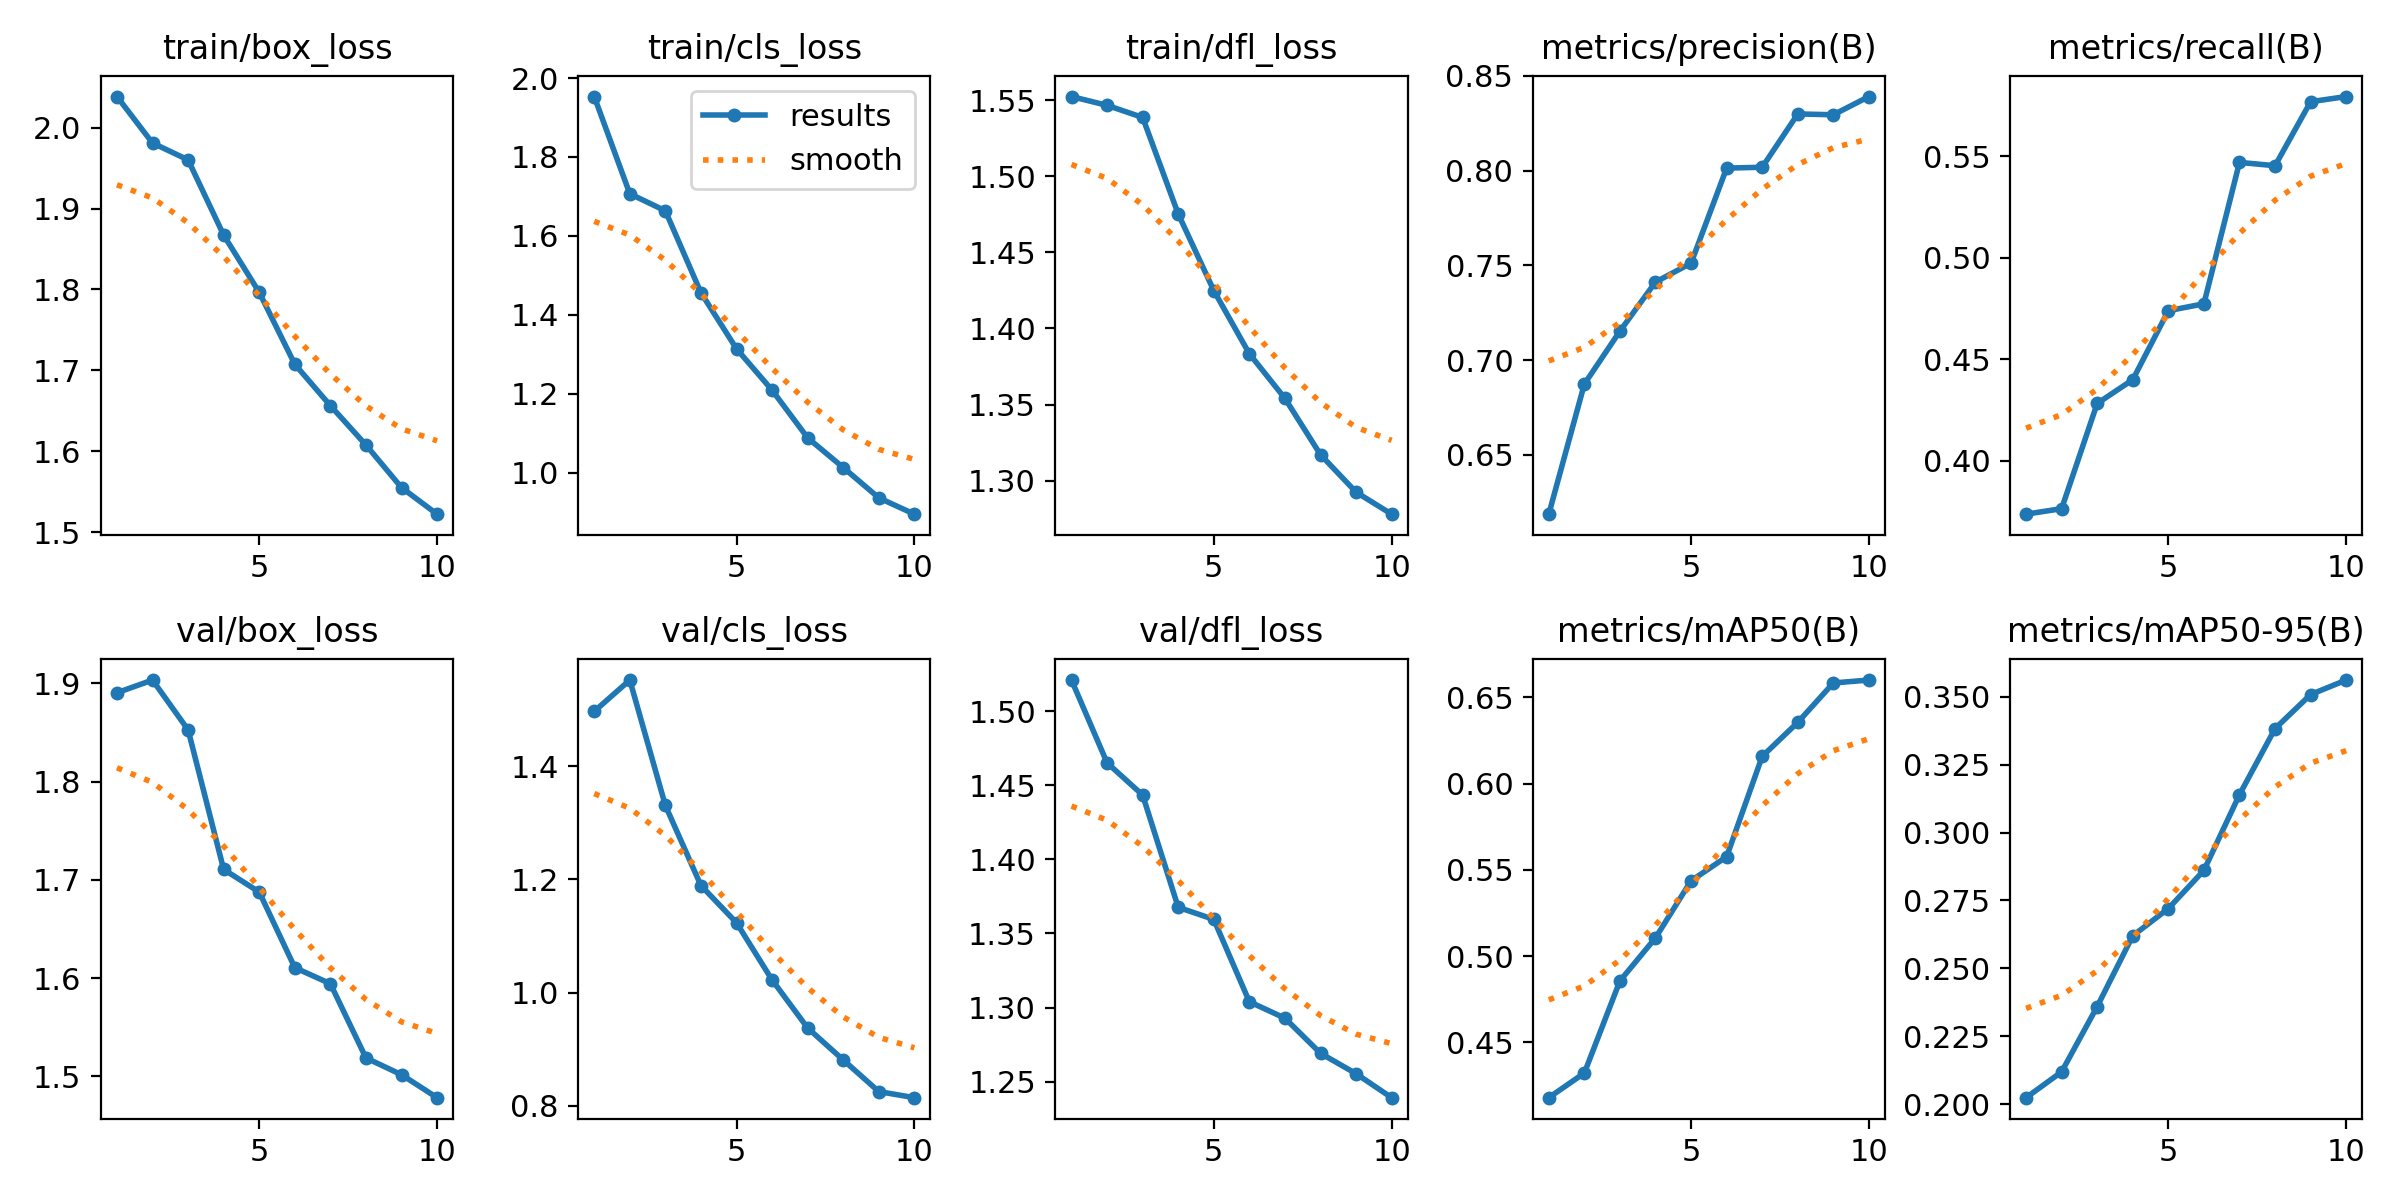
\includegraphics[width=\textwidth,height=0.34\textheight,keepaspectratio]{imglib/face_model_lab/yolo_results.png}
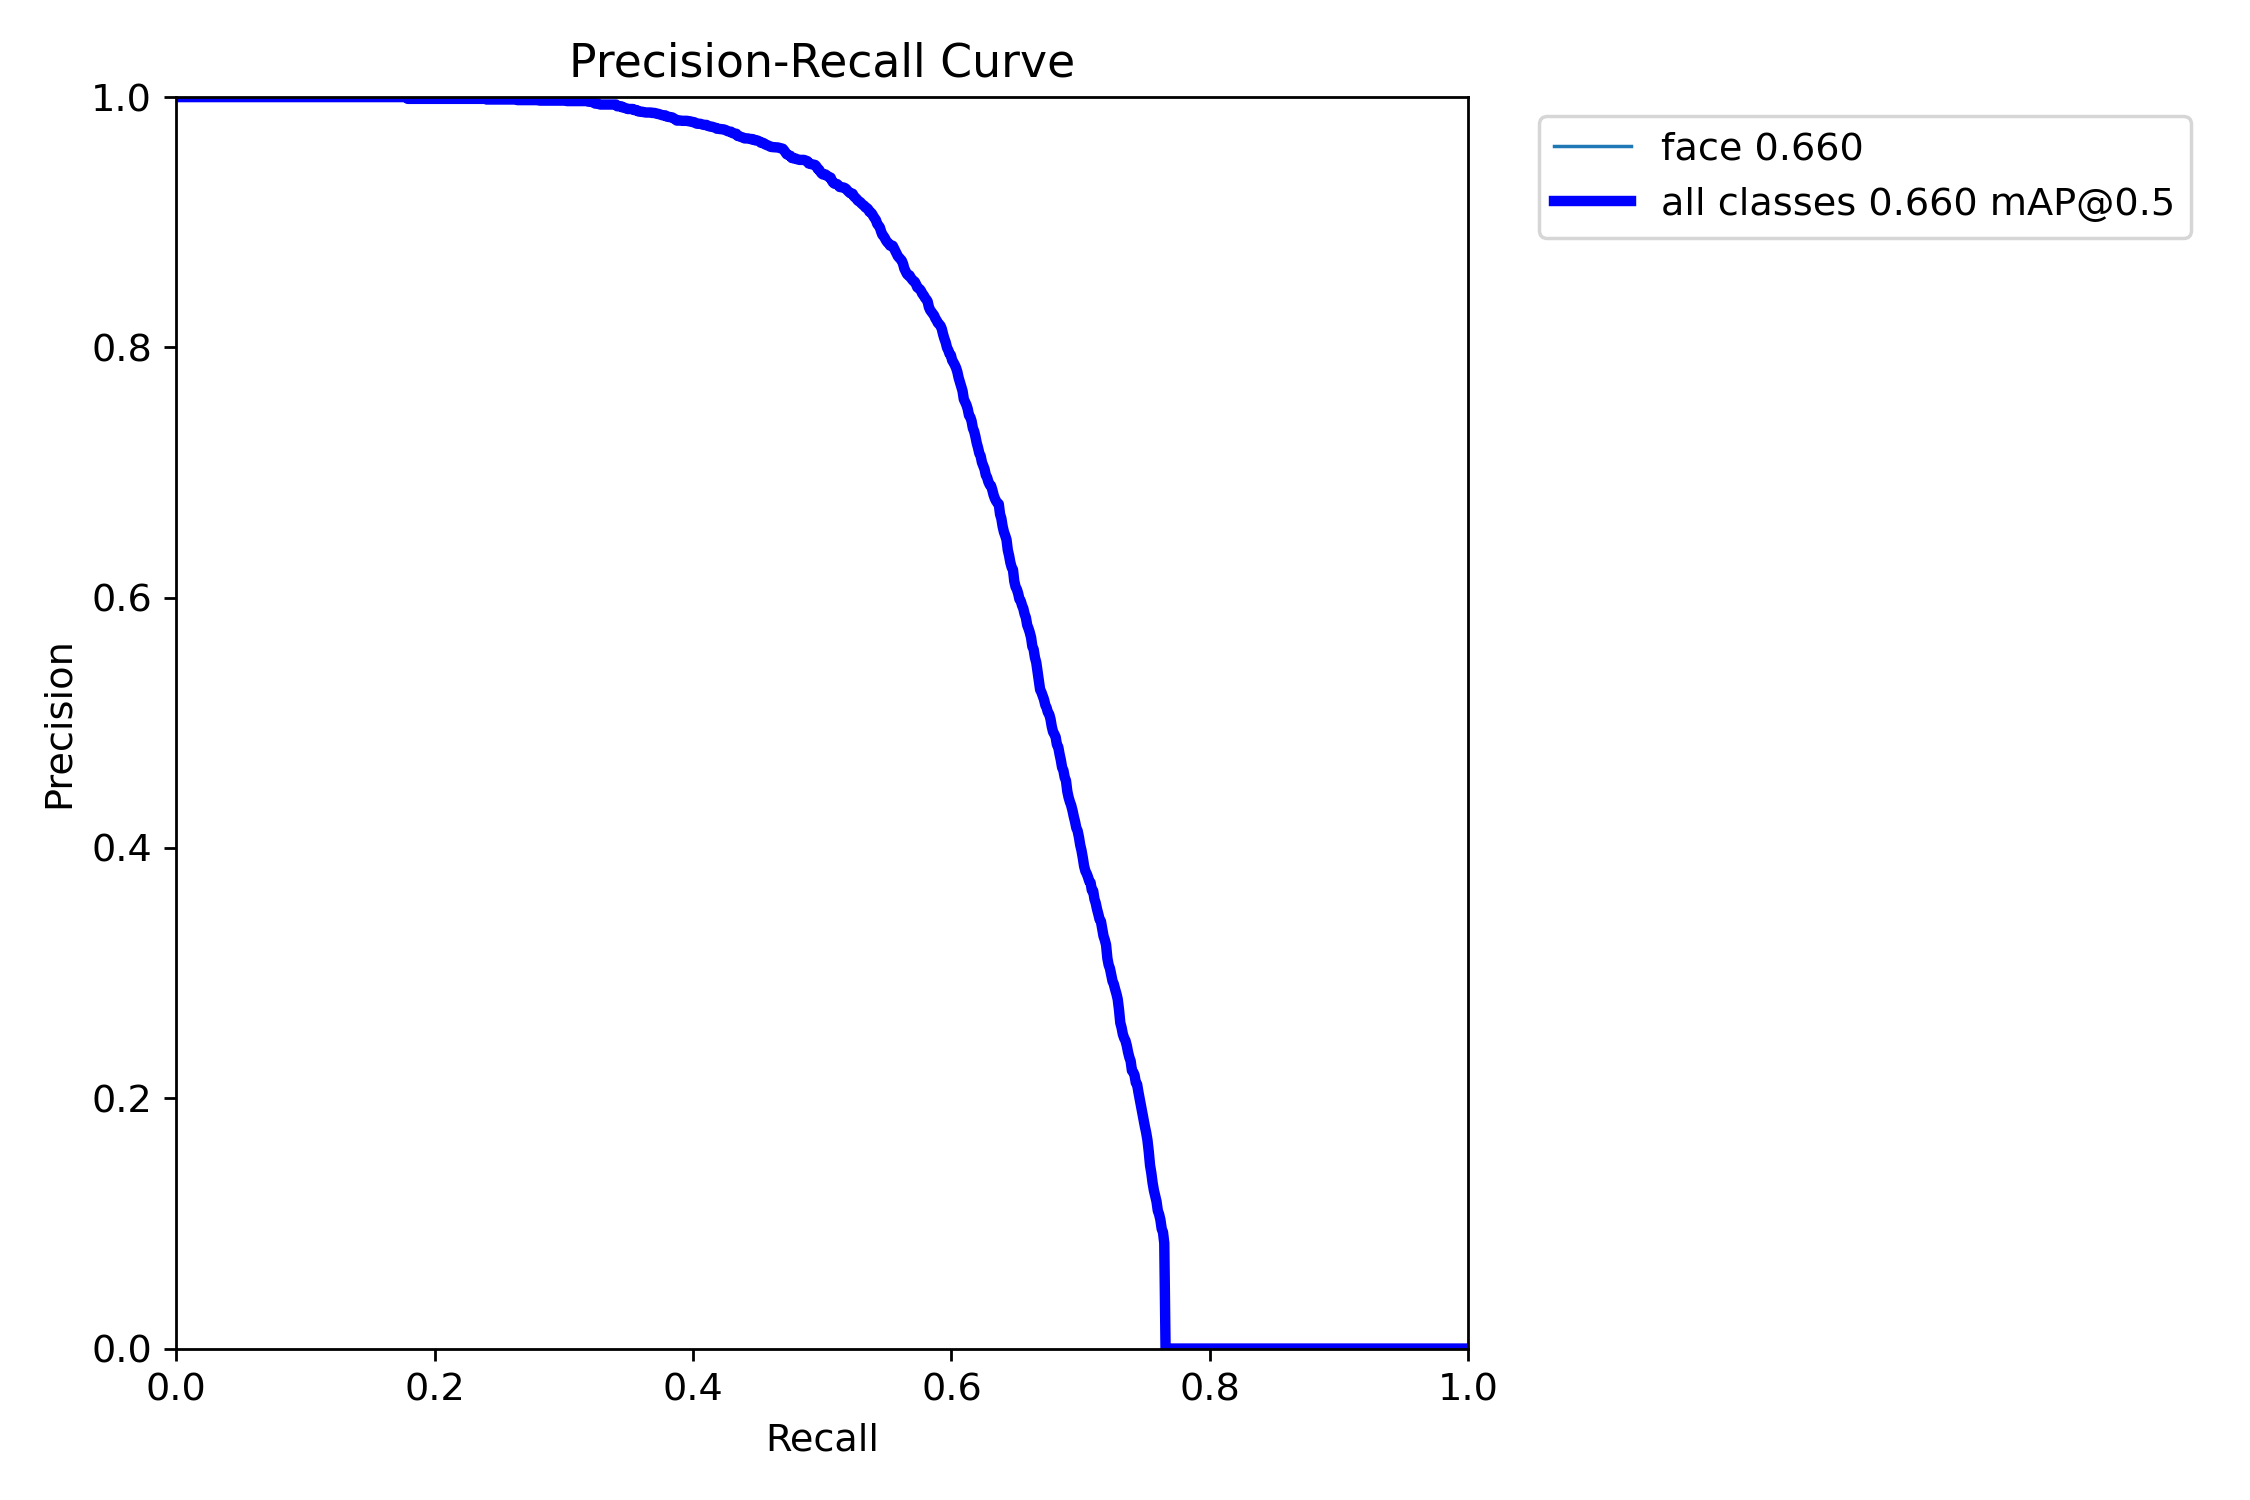
\includegraphics[width=\textwidth,height=0.27\textheight,keepaspectratio]{imglib/face_model_lab/yolo_box_pr_curve.png}
\end{column}
\begin{column}{0.48\textwidth}
\begin{itemize}
    \item FCOS ist der Recall-Sieger und damit die staerkste Wahl fuer maximale Abdeckung.
    \item YOLOv8m ist schneller, liefert viele Run-Artefakte und passt gut zur Video-Pipeline.
    \item Die Modellentscheidung ist deshalb zweigeteilt: Qualitaet gegen operative Einfachheit.
\end{itemize}
\begin{mynote}[Uebergabe]
Jetzt schauen wir, wie aus der Detektion geblurrte Videos entstehen.
\end{mynote}
\end{column}
\end{columns}
\end{frame}
